\documentclass[12pt,letterpaper]{article}
\usepackage[utf8]{inputenc}
\usepackage[spanish]{babel}
\usepackage{graphicx}
\usepackage[left=2cm,right=2cm,top=2cm,bottom=2cm]{geometry}
\usepackage{graphicx} % figuras
% \usepackage{subfigure} % subfiguras
\usepackage{float} % para usar [H]
\usepackage{amsmath}
%\usepackage{txfonts}
\usepackage{stackrel} 
\usepackage{multirow}
\usepackage{enumerate} % enumerados
\usepackage{changepage}
\usepackage{amsmath}
\usepackage[all]{xy}
\renewcommand{\labelitemi}{$-$}
\renewcommand{\labelitemii}{$\cdot$}

% \author{}
% \title{Caratula}
\begin{document}

% Fancy Header and Footer
% \usepackage{fancyhdr}
% \pagestyle{fancy}
% \cfoot{}
% \rfoot{\thepage}
%

% \usepackage[hidelinks]{hyperref} % CREA HYPERVINCULOS EN INDICE

% \author{}
\title{Caratula}

\begin{titlepage}
\begin{center}
\large{UNIVERSIDAD PRIVADA DE TACNA}\\
\vspace*{-0.025in}
\begin{figure}[htb]
\begin{center}
\vspace{\baselineskip}

\includegraphics[width=4.5cm]{./Imagenes/logo}
\end{center}
\end{figure}
\vspace*{0.15in}
INGENIERIA DE SISTEMAS  \\

\vspace*{0.5in}
\begin{large}
TITULO:\\
\end{large}

\vspace*{0.1in}
\begin{Large}
\textbf{INFORME LABORATORIO 06} \\
\end{Large}

\vspace*{0.3in}
\begin{Large}
\textbf{CURSO:} \\
\end{Large}

\vspace*{0.1in}
\begin{large}
BASE DE DATOS II\\
\end{large}

\vspace*{0.3in}
\begin{Large}
\textbf{DOCENTE:} \\
\end{Large}

\vspace*{0.1in}
\begin{large}
 ING. Patrick Cuadros Quiroga\\
\end{large}

\vspace*{0.2in}
\vspace*{0.1in}
\begin{large}
Integrantes: \\
\vspace{\baselineskip}
\begin{flushleft}
Condori Gutierrez, Flor de Maria            	\hfill	(2015053227) \\
Salamanca Contreras, Fiorella Rosmery		\hfill	(2015053237) \\
\end{flushleft}
\end{large}
\end{center}

\end{titlepage}

\tableofcontents % INDICE
\thispagestyle{empty} % INDICE SIN NUMERO
\newpage
\setcounter{page}{1} % REINICIAR CONTADOR DE PAGINAS DESPUES DEL INDICE

\section{Respuesta al ejecutar los siguientes comandos} 
\vspace{\baselineskip}
¿Qué sucede al ejecutar los siguientes comandos?
\begin{center}
	
\includegraphics[width=8cm]{./Imagenes/1} 
\end{center}

\begin{itemize}
	\item STARTUP OPEN
\end{itemize}
\begin{adjustwidth}{0.40in}{0.0in}
	Una base de datos Oracle puede estar en uno de estos cuatro estados:
	OPEN: La base de datos está completamente funcional. Para ello se abren los archivos de datos y los Redo Log y se comprueba la consistencia de los datos.\\ \\
	Este es el valor por defecto para arrancar, montar y abrir una base datos.\\ \\
	Abrir la base de datos incluyendo las siguientes tareas:	
	\begin{itemize}
		\item[$*$] Apertura de los archivos de datos en línea.
		\item[$*$] Apertura de los archivos de registro de rehacer en línea.\\
\\
	\end{itemize}		
\end{adjustwidth}

\begin{itemize}
	\item STARTUP MOUNT 
\end{itemize}
\begin{adjustwidth}{0.40in}{0.0in}
	Una base de datos Oracle puede estar en uno de estos cuatro estados:
	MOUNT: Al estado anterior se añade la lectura de los archivos de control que permiten determinar cómo se ha de preparar la instancia. Se buscan los archivos de datos y los Redo Log, comprobando su existencia en las rutas marcadas por el archivo de control.\\ \\
	En este estado podemos conectar (como administradores) y realizar tareas como:
	\begin{itemize}
		\item[$*$] Cambio del nombre de los archivos de datos.
		\item[$*$] Activar el modo ARCHIVELOG.
		\item[$*$] Recuperación de la base de datos
		\item[$*$] En definitiva, tareas sobre los archivos de la base de datos ya que aun no se han abierto sus datos.	\\
\\
	\end{itemize}
	Arrancamos la base de datos montada, normalmente se usa en modo para tareas de mantenimiento.	
\end{adjustwidth}

\begin{itemize}
	\item STARTUP NOMOUNT 
\end{itemize}
\begin{adjustwidth}{0.40in}{0.0in}
	Una base de datos Oracle puede estar en uno de estos cuatro estados: \\ \\
	NOMOUNT: La instancia de base de datos está latente en memoria, con los procesos comunes funcionando. Se abre el archivo de parámetros, se asigna en memoria el espacio para la SGA, se lanzan los procesos en segundo plano, se abren los archivos de traza y alerta.\\ \\
	Arrancamos la base de datos (instancia) pero sin montarla, se suele usar la fase de creación de una base de datos.\\ \\
	Una instancia se inicia normalmente solo en modo Nomount durante:
	\begin{itemize}
		\item[$*$] Creación de base de datos
		\item[$*$] Recreación de archivos de control.
		\item[$*$] Ciertos escenarios de copia de seguridad y recuperación.\\

	\begin{center}
		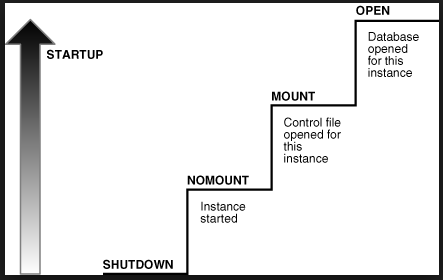
\includegraphics[width=15.3cm]{./Imagenes/startup}
	\end{center}

	\end{itemize}
\end{adjustwidth}

\begin{itemize}
	\item STARTUP FORCE  
\end{itemize}
\begin{adjustwidth}{0.40in}{0.0in}
	Arranque con un fichero de parámetros distinto al habitual o localizado en una situación diferente a donde se encuentra por defecto.\\ \\
	Si la base de datos está abierta, FORCE apaga la base de datos con una SHUTDOWN ABORT declaración antes de volver a abrirla. Si la base de datos está cerrada, entonces FORCE abre la base de datos.\\ \\
	Puede usar la opción de inicio de STARTUP FORCE si tiene dificultades para iniciar la base de datos de una manera normal. Por ejemplo, si un servidor de base de datos perdió energía y la base de datos se detuvo bruscamente, puede dejar la base de datos en un estado en el que sea necesario un inicio de STARTUP FORCE.\\ \\
	Este tipo de inicio normalmente no debería ser requerido, pero puede usarse si un inicio normal no funciona. STARTUP FORCE realiza un aborto de apagado y luego reinicia la base de datos.
\end{adjustwidth}

\begin{itemize}
	\item STARTUP RESTRICT  
\end{itemize}
\begin{adjustwidth}{0.40in}{0.0in}
	Es un modo especial de trabajo en el que la base de datos está abierta, pero solo se permite el acceso a usuarios con permiso RESTRICTED (lo poseen los administradores) para hacer tareas especiales de administración. Uso:\\
	\begin{center}
		\textbf{\large STARTUP RESTRICTED}		
	\end{center}
	\vspace{\baselineskip}
	Si la instancia ya estaba abierta es:\\
	\begin{center}
		\textbf{\large ALTER SYSTEM ENABLE RESTRICTED SESSION;}		
	\end{center} 

	Y si lo que queremos es desactivar el modo restringido para pasar a modo normal:\\
	\begin{center}
		\textbf{\large ALTER SYSTEM DISABLE RESTRICTED SESSION;}		
	\end{center}
	\vspace{\baselineskip}
	Arrancamos la base de datos en modo restringido, solo usuario que tengan privilegios de CREATE SESSION y RESTRICTED SESSION podrán conectarse.\\ \\
	La opción STARTUP RESTRICT inicia la base de datos y la coloca en modo ABIERTO, pero da acceso solo a los usuarios que tienen el privilegio RESTRICTED SESSION. Es posible que desee abrir una base de datos utilizando la opción RESTRINGIDA cuando desee realizar el mantenimiento de la base de datos mientras esté abierta, pero asegúrese de que los usuarios no puedan conectarse y realizar trabajos en la base de datos.\\ \\
	Es posible que también desee abrir la base de datos utilizando la opción RESTRINGIDA para realizar exportaciones o importaciones de la base de datos y garantizar que ningún usuario acceda al sistema durante estas actividades. Una vez que haya terminado con su trabajo, puede deshabilitar la sesión restringida, ALTERAR LA SESIÓN RESTRINGIDA DEL SISTEMA, para que todos puedan conectarse a la base de datos.\\
\\
	
\end{adjustwidth}

\begin{itemize}
	\item STARTUP RECOVER  
\end{itemize}
\begin{adjustwidth}{0.40in}{0.0in}
	Especifica que la recuperación de medios se debe realizar, si es necesario, antes de iniciar la instancia. STARTUP RECOVER tiene el mismo efecto que emitir el comando RECOVER DATABASE e iniciar una instancia. Solo la recuperación completa es posible con la opción RECUPERACIÓN.\\ \\
	La recuperación continúa, si es necesario, como si AUTORECOVERY estuviera en ON, independientemente de si AUTORECOVERY está habilitado o no. Si no se encuentra un archivo de registro de rehacer en la ubicación esperada, la recuperación continúa como si AUTORECOVERY estuviera deshabilitado, al indicarle la ubicación sugerida y el nombre de los archivos de registro posteriores que deben aplicarse.\\
\\
\end{adjustwidth}

\begin{itemize}
	\item SHUTDOWN NORMAL   
\end{itemize}
\begin{adjustwidth}{0.40in}{0.0in}
	Una instancia cuando es arrancada, hasta estar disponible atraviesa todos los estados anteriores.\\ 
	El comando de apagado de la instancia es SHUTDOWN, su sintaxis:\\ \\
	NORMAL: Modo en el que no se admiten más conexiones a la base de datos, pero las actuales se mantienen. Cuando se cierre la última sesión, la base de datos pasará a estar cerrada (SHUTDOWN), pero, hasta entonces, seguirá abierta. Al cerrar se fuerza un checkpoint y se graban todos los datos del búfer, además de cerrarse los archivos.\\ \\
	Caracteristicas:
	\begin{itemize}
		\item[$*$] Espera a que los usuarios conectados actualmente finalicen TODAS las operaciones.
		\item[$*$] Evita nuevas conexiones. Los usuarios que intentan conectarse reciben el mensaje "Shutdown in progress".
		\item[$*$] Cierra y desmonta la B.D. Cierra la SGA para los procesos background.
		\item[$*$] No necesita recuperacion al arrancar la base de datos.\\ \\
	\begin{center}
		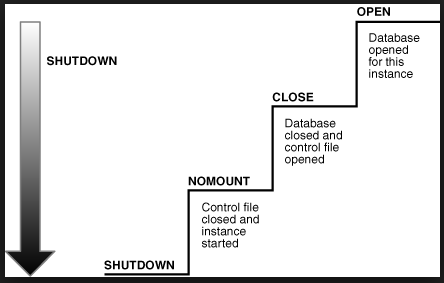
\includegraphics[width=15.3cm]{./Imagenes/shutdown}
	\end{center}
	\end{itemize}	
\end{adjustwidth}

\vspace{\baselineskip}
\vspace{\baselineskip}


\end{document}
